% =====================================================================
%  Assessment 2 poster. A0 PORTRAIT (841 x 1189 mm) -- the usual European
%  default, but the brief does not state a size. If the guidelines specify
%  A1 or landscape, change the geometry line only; everything scales.
%
%  Numbers are copied from report/main.tex, which generates them from
%  results/*.csv. If a result changes, re-run src/make_tables.py, check the
%  report, then update here.
%
%  THIS IS THE THING YOU STAND NEXT TO. Whoever presents has to answer
%  "what is an integrated calibration index?" and "why is the Fine-Gray risk
%  set weighted that way?" without the poster's help. Rewrite the wording so
%  it is yours before you print it.
% =====================================================================
\documentclass[final]{article}
\usepackage[a0paper,portrait,margin=4cm]{geometry}
\usepackage[T1]{fontenc}
\usepackage[utf8]{inputenc}
\usepackage{lmodern}
\usepackage{multicol}
\usepackage{graphicx}
\usepackage{booktabs}
\usepackage{xcolor}
\usepackage[most]{tcolorbox}
\usepackage{microtype}
\pagestyle{empty}
\setlength{\parindent}{0pt}

\definecolor{su}{HTML}{1B4965}
\definecolor{accent}{HTML}{B5451B}
\definecolor{soft}{HTML}{EEF2F5}

\renewcommand{\familydefault}{\sfdefault}

% body type for A0
\makeatletter
\renewcommand\normalsize{\@setfontsize\normalsize{39}{48}}
\makeatother
\normalsize

\newtcolorbox{panel}[1]{
  enhanced, colback=white, colframe=su, boxrule=1.2pt, arc=3mm,
  fonttitle=\bfseries\fontsize{46}{55}\selectfont, coltitle=white,
  colbacktitle=su, title={#1}, left=6mm, right=6mm, top=4mm, bottom=4mm,
  before skip=3mm, after skip=3mm}

\newtcolorbox{hilite}{
  enhanced, colback=soft, colframe=accent, boxrule=1.6pt, arc=3mm,
  left=6mm, right=6mm, top=5mm, bottom=5mm, before skip=3mm, after skip=3mm}

\newcommand{\bignum}[2]{{\fontsize{64}{72}\selectfont\bfseries\color{accent}#1}\\[1mm]{\fontsize{32}{39}\selectfont #2}}

\begin{document}

% ---------------- header ----------------
\begin{center}
{\fontsize{88}{100}\selectfont\bfseries\color{su}
Ranking, Calibration and Cost in\\[3mm] Competing-Risks Survival Models}\\[6mm]
{\fontsize{42}{50}\selectfont A Common-Protocol Benchmark on 550{,}000 Mortgages}\\[8mm]
{\fontsize{38}{46}\selectfont Amirreza Sadraei \quad\textbullet\quad Ali Emre Nebiler \quad\textbullet\quad Filip Becic}\\[3mm]
{\fontsize{39}{48}\selectfont Department of Computer and Systems Sciences, Stockholm University}
\end{center}
\vspace{4mm}
{\color{su}\hrule height 3pt}
\vspace{8mm}

\begin{multicols}{3}

% ================= COLUMN 1 =================
\begin{hilite}
{\fontsize{46}{55}\selectfont\bfseries\color{su} The question}\\[4mm]
Deep competing-risks models are usually compared on how well they
\textbf{rank} borrowers. A lender provisioning against loss needs the
\textbf{probability}. We tested whether the ranking advantage holds when both
are measured.
\end{hilite}

\begin{panel}{Why it matters}
A mortgage ends in one of three ways: default, prepayment or maturity. Once
one happens the other two cannot, which is what makes this a competing-risks
problem.

\vspace{4mm}
IFRS 9 requires a probability of default at each future date, and the reserve is
computed from it. A model can order borrowers correctly and still get those
probabilities wrong.
\end{panel}

\begin{panel}{Data}
{\raggedright Freddie Mac Single-Family Loan-Level Dataset, 50{,}000-loan
samples per vintage.\par}

\vspace{4mm}
\begin{tabular}{@{}lrr@{}}
\toprule
Cohort & Train & Test \\
\midrule
Post-crisis & 2013--15 & 2016--18 \\
Crisis & 2005--06 & 2007--09 \\
\bottomrule
\end{tabular}

\vspace{5mm}
\begin{center}
\bignum{20.6\% vs 95.5\%}{censoring, counting prepayment as an event\\versus censoring it}
\end{center}

\vspace{3mm}
Dirick et al.\ report 20--85\% and 94.56--98.16\% across ten European
consumer-credit portfolios. Our figures fall inside both ranges on US mortgages
from a later decade.
\end{panel}

\begin{panel}{Protocol}
Every model returns a cumulative incidence function per cause, so all five are
scored on all three metrics.

\vspace{4mm}
\textbf{Models} \ Aalen--Johansen (null), cause-specific Cox, Fine--Gray, random
survival forest, DeepHit

\vspace{1mm}
\textbf{Ranking} \ IPCW time-dependent AUC

\vspace{1mm}
\textbf{Calibration} \ integrated calibration index, integrated Brier

\vspace{1mm}
\textbf{Cost} \ fit and predict seconds

\vspace{1mm}
\textbf{Splits} \ vintage-ordered, not random

\vspace{1mm}
\textbf{Budget} \ 20 DeepHit configs, 8 forest, fixed in advance, validated
out-of-time

\vspace{1mm}
\textbf{Inference} \ paired bootstrap, $B{=}500$, two-sided, $\alpha$ fixed at
0.05, Bonferroni across three metric families
\end{panel}

% ================= COLUMN 2 =================
\begin{panel}{1. The advantage reverses with regime}
AUC at 60 months, default:

\vspace{4mm}
\begin{tabular}{@{}lrr@{}}
\toprule
& Crisis & Post-crisis \\
\midrule
DeepHit (tuned) & \textbf{0.8538} & 0.7280 \\
Cause-specific Cox & 0.8346 & \textbf{0.7372} \\
\midrule
Difference & $+0.0192$ & $-0.0091$ \\
\bottomrule
\end{tabular}

\vspace{5mm}
Both are significant under the paired bootstrap. The crisis win is
harder to read than it looks: refitting Cox on resamples of its own training
vintages moves its AUC by $\pm0.0159$, against 0.0035 for DeepHit. Here the
classical models are the less stable ones.

\vspace{4mm}
Calibration behaves the same way in both regimes: DeepHit's calibration index is
0.0040 worse than Cox's in each.
\end{panel}

\begin{panel}{2. DeepHit against a random forest}
\begin{center}
\bignum{$p=0.97$ \ \ $p=0.79$}{DeepHit vs tuned random survival forest, AUC,\\crisis and post-crisis}
\end{center}

\vspace{3mm}
Neither difference reaches significance, and both are smaller than DeepHit's
spread across seeds. On crisis \textbf{prepayment} the forest is ahead on both,
0.685 against 0.620 on AUC and 0.154 against 0.236 on calibration.
\end{panel}

\begin{panel}{3. What the loss weight does}
DeepHit's loss is $\alpha\cdot$likelihood $+\ (1-\alpha)\cdot$ranking. Averaging
our 40 tuning configurations by $\alpha$, validation AUC rises from 0.658 at
$\alpha{=}0.1$ to 0.776 at $\alpha{=}1.0$, a strong monotone effect.

\vspace{5mm}
We then varied $\alpha$ alone, holding architecture, dropout, learning rate,
batch size and bin count fixed, over five seeds and both cohorts:

\vspace{4mm}
\begin{tabular}{@{}llrr@{}}
\toprule
Cause & Cohort & $\Delta$AUC & seed sd \\
\midrule
Default & crisis & $+0.0075$ & 0.0033 \\
Default & post & $+0.0005$ & 0.0018 \\
Prepay & crisis & $\mathbf{-0.0673}$ & 0.0103 \\
Prepay & post & $\mathbf{+0.0386}$ & 0.0062 \\
\bottomrule
\end{tabular}

\vspace{5mm}
$\Delta$ is the change from $\alpha{=}0.1$ to $\alpha{=}1$. Three of the four
cells exceed the seed standard deviation and they disagree about direction:
crisis prepayment loses 0.067 of AUC where post-crisis prepayment gains 0.039.

\vspace{5mm}
In the search $\alpha$ varied together with depth, dropout and batch size, so the
pooled table measured all of them at once. \textbf{We had written the
opposite conclusion before we ran the controlled version.}
\end{panel}

% ================= COLUMN 3 =================
\begin{panel}{4. Where the calibration gap comes from}
\begin{tabular}{@{}lrr@{}}
\toprule
Calibration index & Crisis & Post-crisis \\
\midrule
Raw & 0.0209 & 0.0318 \\
Recalibrated (train) & 0.0164 & 0.0297 \\
Recalibrated (oracle) & \textbf{0.0053} & \textbf{0.0082} \\
\bottomrule
\end{tabular}

\vspace{5mm}
We estimated a per-horizon rescaling two ways. Fitted on the training
vintages, which is what a lender has at scoring time, it changes very little and
in 10 of 16 cells makes calibration worse. Fitted on the test vintages it cuts
the error by a median factor of 4.2.

\vspace{4mm}
\textbf{It works when it is estimated on the vintages it will be applied to, and
those are the ones a lender does not have yet.}
\end{panel}

\begin{panel}{Calibration at 60 months, crisis cohort}
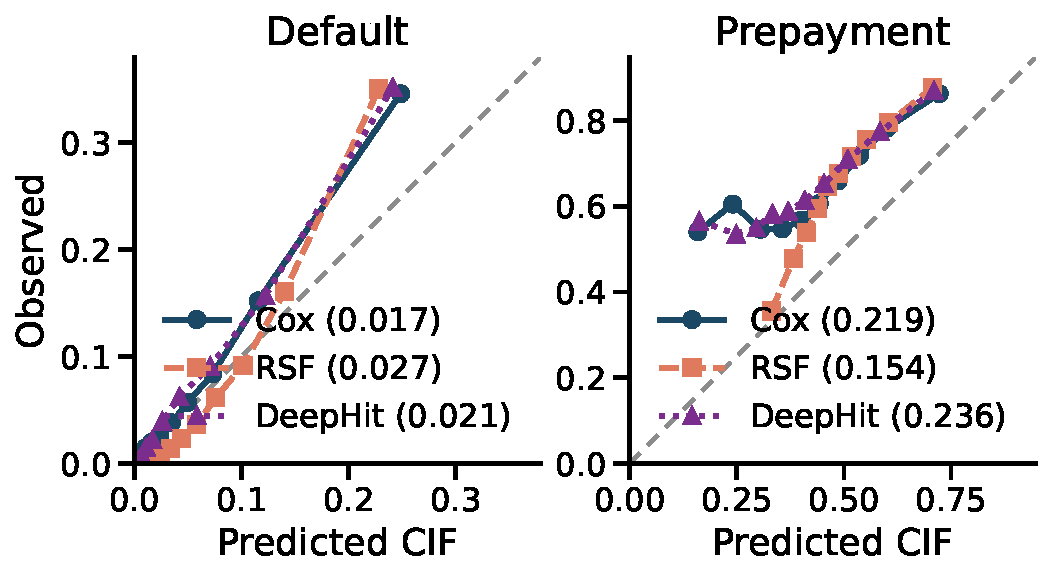
\includegraphics[width=\linewidth]{fig_calibration_poster}

\vspace{3mm}
{\fontsize{32}{39}\selectfont Deciles of predicted risk against the
Aalen--Johansen estimate. All three models sit above the diagonal, and the gap
is far wider for prepayment.}
\end{panel}

\begin{panel}{Cost}
\begin{center}
\bignum{$\approx 2{,}000\times$}{DeepHit (59\,s) versus Fine--Gray (0.03\,s)\\per fit, 150{,}000 loans}
\end{center}
The DeepHit search added 14.4 minutes across the two cohorts. The classical
models have no search to run.
\end{panel}

\begin{panel}{What we cannot claim}
All results come from one family of US agency mortgages. Variability comes from
only five bootstrap replicates. Covariates are
observed at origination, so we have no time-varying macroeconomic variables. Our
recalibration is a marginal rescaling rather than the per-cause procedures of
Alberge et al.\ (2026). With 150{,}000 test loans most differences reach
significance, so we report effect sizes alongside $p$-values.
\end{panel}

\begin{hilite}
\begin{center}
{\fontsize{46}{56}\selectfont\bfseries\color{su}
DeepHit ranks better in one\\[2mm] of two regimes, and is\\[2mm]
worse calibrated in both.}

\vspace{6mm}
{\fontsize{30}{36}\selectfont Code: \texttt{github.com/ar-sadraei/rtds-project}\\[2mm]
Data: Freddie Mac SFLLD, free on registration}
\end{center}
\end{hilite}

\end{multicols}
\end{document}
